\documentclass[12pt, a4paper]{article}
\usepackage[nottoc,numbib]{tocbibind}
\usepackage[T1]{fontenc}
\usepackage{tgtermes}
\usepackage{subfiles}
\usepackage{graphicx}


\linespread{1.25}
\newtheorem{definition}{Definition}


\begin{document}
  \subfile{sections/titlepages}

  \tableofcontents
  \newpage

  \section{Introduction}
  \newpage

  \section{Background}
  \subsection{Fundamentals of Deep Learning}

  Given that deep learning lays at the foundation of the thesis and the web application, this chapter will provide an overview of the core concepts.

  \subsubsection{Introduction}
  
  Artificial intelligence (AI), originally coined as a term and founded as an academic discipline in the 1950s \cite{a5}, has become a buzzword not only in the domain of computer science, but also in popular culture. The growth in popularity and general interest is owed to the accelerated technological advancements and exponential increase in the volumes of data, which fueled the progression of AI from bare theory to a gradual actuality.

  There is no singular universally accepted definition for artificial intelligence. This term generated a considerable amount of differences and confusion among specialists\cite{a6}. There are numerous proposed definitions, but one that encapsulates to a certain extent a common essence encountered in a fair part of them could be formulated as follows:

  \begin{definition}
    Artificial intelligence (AI) is a branch of computer science, concerned with developing computer programs that approach problems emulating the human model of thinking and its typical processes, such as learning, reasoning and self-correction.
  \end{definition}

  Another term coined also in the 1950s is the one of "machine learning". Machine learning (ML) is a subfield of AI, based on the idea that computers can be programmed to "learn" from data and tackle tasks with minimal human intervention. A definition for this field of study, based on Tom Mitchell's proposal \cite{b1}, is the following one:

  \begin{definition}
    Machine learning (ML) is a branch of computer science and sub-branch of artificial intelligence, which studies the capability of a computer program to learn from experience E with respect to some task T and some performance measure P, improving with experience E its performance on the task T, measured by P.
  \end{definition}
  
  A prevalent subset of machine learning is called deep learning (DL), which approaches problems by means of artificial neural networks. An artificial neural network is an interconnected set of nodes, disposed in multiple layers, which emulates the way in which neurons function in a real neural network. In other words, deep learning algorithms are inspired by how a brain learns. According to \cite{a7}, deep learning can be formally defined as below.

  \begin{definition}
    Deep learning (DL) is a class of machine learning algorithms that: (1) use a cascade of multiple layers of nonlinear processing units for feature extraction and transformation. Each successive layer uses the output from the previous layer as input, (2) learn multiple levels of representations that correspond to different levels of abstraction; the levels form a hierarchy of concepts.
  \end{definition}

  The previously cited source, further explains that the reason deep learning has gained so much popularity in the last decades and bore out to be so powerful, is not particularly owing to its resemblance with human-like thinking, but primarily due to its deep, multi-layered architecture. Until recently, most machine learning algorithms had exploited shallow-structured architecture, which do not consist of more than one or two layers of nonlinear feature transformation. Although this plainer architecture proved efficacy in many simple and well-constrained problems, it might cause complications in some more complex applications.

  Some of the large novel fields in which deep learning was successfully implemented and notably pushed the boundaries include speech recognition, audio processing, natural language processing (e.g. language translation, search results, smart assistants, text analysis), computer vision (e.g. object detection, image classification, segmentation), information retrieval, multi-modal and multi-task learning, and so forth. Out of these, what is of chief interest within this thesis and web application, which aim to come to grips with the issue of fake news detection, is natural language processing.

  \begin{definition}
    Natural language processing (NLP) is a field of study at the intersection of artificial intelligence and linguistics, which is comprised of a range of computational techniques for analyzing and representing human language \cite{a8}.
  \end{definition}

  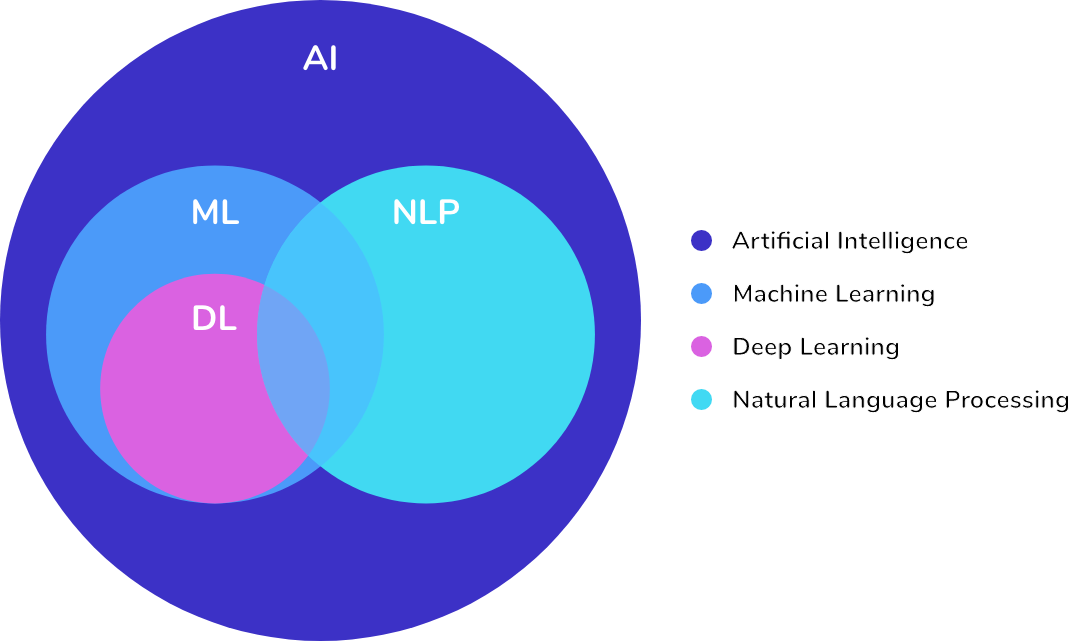
\includegraphics[width=\textwidth,height=\textheight,keepaspectratio]{images/ai-dl-ml-nlp-diagram.png}

  \subsubsection{More on Deep Learning}
  \subsubsection{More on Natural Language Processing}

  \subsection{Fake News}
  Fake news is not simply a product of the last decades. It has been part of humanity for at least centuries. Its first significant outburst dates back to 1400s, when the printing press was invented. Ever since then, fabricated news have been more and more weaponized to manipulate people at increasingly larger scales. In 1835, The New York Sun published 6 articles presenting the discovery of life on the moon. Both World Wars were heavily marked by propaganda, and false and misleading news \cite{a4}. And more recently, the US 2016 presidential elections and the COVID-19 pandemic were subjects of large amounts of fake news.

  Despite being so widespread, there is no globally agreed definition of the "fake news" term. Nonetheless, many sources provide definitions which have two primary elements in common: authenticity and intent. As for authenticity, fake news contain claims that are factually and verifiably false. As for intent, the major purpose of fake news is to deceive the consumers \cite{a2}. That being said, a concise definition of fake news could be formulated in the following manner:

  \begin{definition}
    By fake news we mean any news item that is deliberately and factually untrue and misleading.
  \end{definition}

  \subsection{Fake News Detection}
  Fake News Detection represents a new area of study. On the one hand, it emerged thanks to the continuous advancements in Artificial Intelligence and, specifically, Deep Learning. On the other hand, it appeared as virtually a necessity, given the recent escalation of the fake news phenomenon, on account of the simultaneous raise of digital media.

  Digital and social media are environments in which the dissemination of information is more facile and rapid than at any point in history. Fabricated news have been heavily published and shared as a means of deception, on subjects of high impact, such as the 2016 US presidential elections and the COVID-19 pandemic.

  At present, there are multiple fake news identification resources. They each contribute in various manners to validating the veracity of news and debunking rumours, hoaxes, conspiracies.


  \subsection{Related Work}
  \newpage


  \section{Application Development}
  
  \section{Conclusion}
  \newpage

  \bibliographystyle{unsrt}
  \bibliography{sources}
  \nocite{*}
\end{document}